%Correct the file name.
%X: book number
%Y: part number
%ZZZ: page number in three digits. So page 3 would be 003.

\documentclass[11pt]{amsbook}

\usepackage{../HBSuerDemir}	
\begin{document}

% ++++++++++++++++++++++++++++++++++++++
\hPage{b1p2/506}
% ++++++++++++++++++++++++++++++++++++++

	\begin{hEnumerateAlpha}
		\item $3(2, 2)$, $4(2, -2)$, $5(-2, 2)$, $2(-2, -2)$

		\item $6(0, 0)$, $6(8, 0)$, $6(8, 8)$, $3(4, 4)$

		\item $2(1, 3)$, $7(4, 2)$, $6(3, -3)$, $8(-4, 2)$, $5(-3, -4)$.
		
 
	\end{hEnumerateAlpha}	
    
   	 \begin{hEnumerateArabic}
 		 \setcounter{enumi}{58}
  		 \item Use PAPPUS' Theorem to  find the centroid of the region of a semicircle 
         	 of radius a.
         	 \item Use PAPPUS' Theorem to find the volume of the torus generated by 
        	 revolving the area of a circle of radius a, about an axis b($>$a) units 
         	 from the center of the circle. \\
	\end{hEnumerateArabic}
    
    	 ANSWERS TO EVEN NUMBERED EXERCISES
    	\begin{hEnumerateArabic}
    		\setcounter{enumi}{35}
    		\item \( \frac{500}{3} \) $\pi$ ($12,25$ + $\sqrt[]{35}$ + 100)
    		\setcounter{enumi}{37}
   			\item 1000 g gr-cm.  
    		\setcounter{enumi}{39}
   			\item 60 kg-cm.
    		\setcounter{enumi}{41}
                \item
    			\begin{enumerate}[label=\alph*)]
				\item $11$$\pi$$\delta$ $r^2$$h^2$ $/ 492$   
        			\item $\pi$$\delta$$r^2$$h(11h/492 + 7k/24)$
   			\end{enumerate}	
    		\setcounter{enumi}{43}
   		\item 840 kg-cm.
    		\setcounter{enumi}{45}
    		\item $kw_1w_2(1/a -1/b)$ kg-m
           	\setcounter{enumi}{47}
           	\item
			 \begin{enumerate}[label=\alph*)]
				\item $M_{ox}$ = $-8 \sqrt[]{2}$ , $M_{oy}$ = $8 \sqrt[]{2}$ , $G(2, -2)$
       			 	\item $M_{0x}$ = $12\pi$ , $M_{0y}$ = $8\pi$ , $G(2, 3)$.
   			 \end{enumerate}	
    		\setcounter{enumi}{49}
                \item
    			\begin{enumerate}[label=\alph*)]
				\item $(1/2, -3/2)$
        			\item $(10, 192/205)$
    			\end{enumerate}
    		\setcounter{enumi}{51}
                \item
    			\begin{enumerate}[label=\alph*)]
				\item $459/20$, $27/4$, $(3/2, 51/10)$
        			\item $243/10$, $27/4$, $(3/2, 27/6)$
    			\end{enumerate}
                \setcounter{enumi}{53}
                \item
            		\begin{enumerate}[label=\alph*)]
				\item $M_{ox} = M_{oy} = 3/20$, $G(9/20, 9/20)$
       			        \item $M_{ox} = 1/4$ , $M_{oy} = (\pi/2 \sqrt[]{2})-1$ , $G(1/4(\sqrt[]{2}-1), (\pi-2 \sqrt[]{2})/2 \sqrt[]{2}( 											\sqrt[]{2}-1)$
    			\end{enumerate}	
               \setcounter{enumi}{55}
               \item
            		\begin{enumerate}[label=\alph*)]
				\item $(12/5 , 3/4)$
                        	\item $(8/5 , 16/7)$
    			\end{enumerate}
               \setcounter{enumi}{57}
               \item 
            		\begin{enumerate}[label=\alph*)]
				\item $(0 , 2/7)$
                  	        \item $(4 , 4)$
                   	        \item $(1/28 , -1/14)$
    			\end{enumerate}
              \setcounter{enumi}{59}
              \item $2\pi^2a^2b$. 
    \end{hEnumerateArabic}

%==== templates ====

%==== environments ====

%\begin{figure}[htb]
%	\centering
%	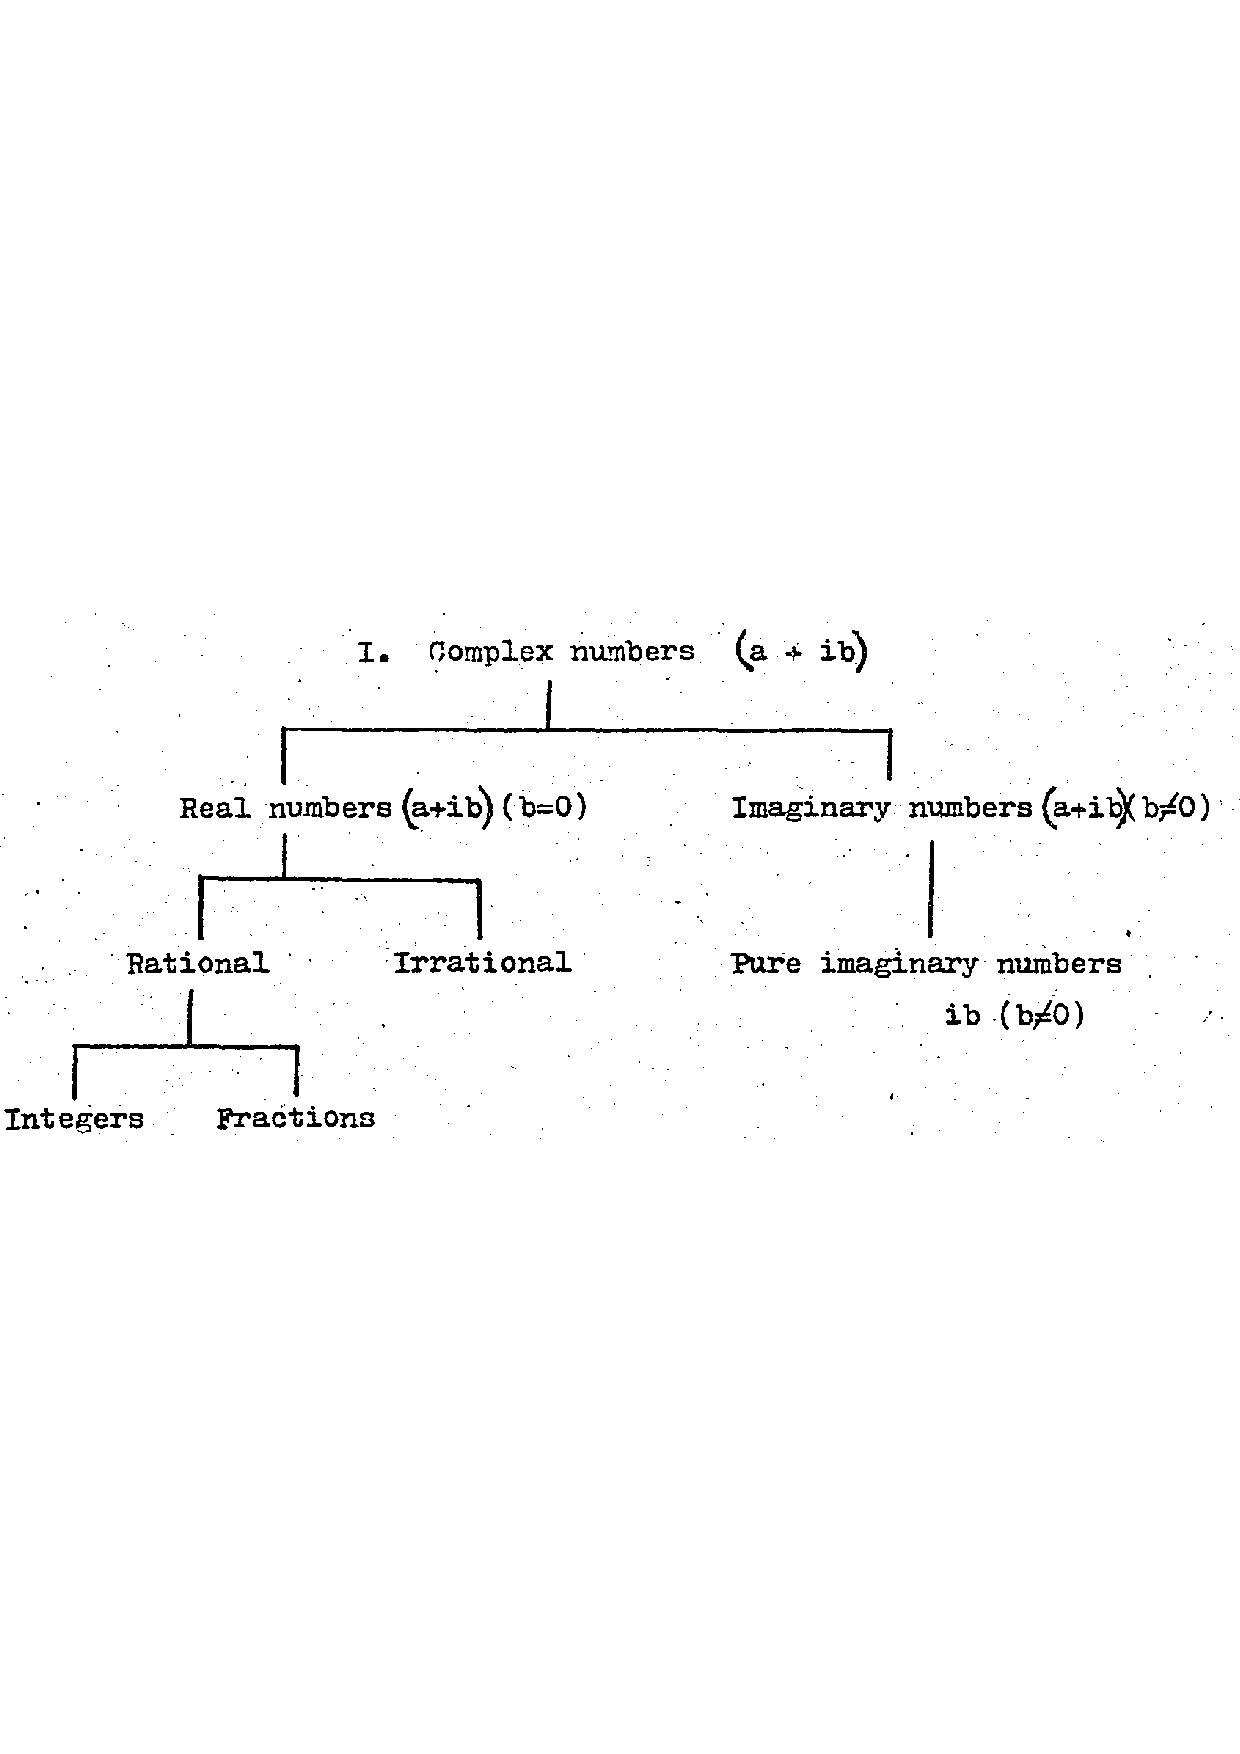
\includegraphics[width=0.9\textwidth]{images/SD-1-1p15A}
%	\caption{Classification of complex numbers}
%	\label{fig:classificationOfComplexNumbersA}
%\end{figure}

%\begin{center}
%\begin{tabular}{cc}
%\end{tabular}
%\end{center}

%\begin{exmp}
%\begin{hSolution}
%\end{hSolution}
%\end{exmp}

%\begin{hEnumerateAlpha}
%\end{hEnumerateAlpha}

%\begin{hEnumerateRoman}
%\end{hEnumerateRoman}

%$
%\begin{bmatrix}
%\end{bmatrix}
%$

%\frac{aaaa}{bbb}
%\frac{a_{n}}{b_{n}}
%\left( aaaa \right)
%\Longrightarrow

%\begin{multicols}{2}
%	bb
%\columnbreak
%	aa
%\end{multicols}

\end{document}  


